\documentclass[11pt, a4paper]{article}
\usepackage[utf8]{inputenc}
\usepackage[sort]{natbib}

\usepackage[english]{babel}
\usepackage{enumitem}
\usepackage{graphicx}
\usepackage{float}
\usepackage[linktoc=all]{hyperref}

\usepackage{etoolbox}

\usepackage{amsmath}
\usepackage{amssymb}
\usepackage{array}
\usepackage{gensymb}

\usepackage{fancyhdr}
\usepackage[table]{xcolor}
\usepackage{color}
\usepackage{colortbl}
\definecolor{lightgray}{gray}{0.9}
\setlength{\columnsep}{0.5cm}


%------------------- Dimensiones -------------------
\usepackage{geometry}
 \geometry{a4paper,total={170mm,257mm},left=15mm,right=15mm,top=20mm,}
%----------------------------------------------------

%------------------- Encabezado y Pie de pág -------------------
\pagestyle{fancy}
\fancyhf{}
\lhead{Técnicas Digitales IV}
\rhead{TP3}
\rfoot{Página \thepage}
%----------------------------------------------------


%----------------------------- Documento -----------------------------------------------
\begin{document}
\begin{titlepage}
 \centering
	
\includegraphics[scale=0.80]{Imagenes/LOGO.jpg} \par
 	\vspace{1cm}
 	{\scshape\LARGE Universidad Tecnológica Nacional \par}
 	{\scshape\large Facultad Regional de Córdoba \par}
 	\vspace{1cm}
	{\bfseries \Large Trabajo Práctico De Laboratorio $N^{\circ} 3$\par}
 	\vspace{1.5cm}

	\begin{tabular}{ll}
		Navarro, Facundo		&	63809 	
	\end{tabular}
	
	\vspace{1cm}
	Curso: 6r4 \\
	Grupo $N^{\circ} 5$
 	\vfill
	{\bfseries \Large Técnicas Digitales IV\par}

	\vspace{1.5cm}
	Docentes: \par
	Ing. Cayuela, Pablo \par
	Ing. Olmedo, Sergio \par

 	\vfill
	{\large \today\par}
\end{titlepage}
	
	
\tableofcontents
\clearpage

\section{Introducción}
En el siguiente trabajo práctico se investigan e implementan protocolos de comunicación síncronos, en donde $R_X$ y $T_X$ operan en conjunto con un señal de $clock$, los cuales son $I^{2}C$, $SPI$, $PS2$.

\section{Personal system version 2 (PS2)}

\section{Serial peripheral interface (SPI)}

\section{Inter intergrated circuit ($I^{2}C$)}
		Es un bus serial de comunicación de 8 bits entre circuitos integrados que se encuentran próximos entre ellos (normalmente en la misma placa). Utiliza tan solo dos cables (mas GND de referencia) y tiene cuatro modos estandarizados de velocidad
		\begin{itemize} \itemsep0em
			\item standard (100 kbps)
			\item fast (400 kbps)
			\item fast-plus (1 Mbps)
			\item high-speed (3,3 Mbps)
		\end{itemize}

		El bus $I^{2}C$ consisten en dos cables, llamados \textit{SCL} (serial clock) y \textit{SDA} (serial data), los cuales interconectan un \textit{master} con un número de unidades \textit{esclavas}.Cada dispositivo en el bus tiene una única dirección y puede operar como transmisor o receptor, poniendo o adquiriendo datos en la linea \textit{SDA}, es decir que esta linea es bidireccional. El clock es unidireccional y es generado por el master, quien además es el encargado de iniciar y finalizar la transferencia de datos. Ejemplos de familias de integrados actualmente fabricados con soporte $I^{2}C$ son: memorias flash y EEPROM, conversores A/D y D/A, circuitos RTC, sensores de temperatura, etc.
		
		Las salidas de SCL y SDA son a  drenador abierto, por lo que son necesarias resistencias del tipo pull-up ($R_{UP}$), normalmente en el rango de los 1,5 a 33 $k\Omega$. El valor de $R_{UP}$ depende de la capacitancia total del nodo, en caso de buses muy largos con muchos esclavos adheridos a él, entonces las resistencias deben ser pequeñas para alcanzar el mínimo ``rise time" definido en la especificaciones del $I^{2}C$.

		El número de dispositivos compartiendo el mismo bus puede alcanzar hasta 128 (direcciones de 7-bit) o 1024 (direcciones de 10-bit). Más de un \textit{master} es permitido, el tal caso el protocolo $I^{2}C$ administra el bus, considerando como master principal al primero que ponga el bajo el voltaje de \textit{SDA}.

		\subsection{Operación de la interfaz $I^{2}C$}
		\paragraph{Diagrama de tiempos.} El diagrama de tiempos de una típica transferencia de datos se muestra en la figura \textcolor{blue}{\textbf{\ref{fig:basic_timing}}}. Ambas líneas están en alto cuando el bus esta en estado ``inactivo". El master inicia la transferencia creando una condición de arranque (S), en la cual SDA cambia de alto a bajo mientras que SCL se mantiene en alto. Luego genera la señal clock sobre SCL. Dependiendo del tipo de transacción, o el maestro o el esclavo seleccionado introducen datos sobre SDA. Los datos deben ser estables cuando SCL este en alto y el cambio de dato solo puede ocurrir cuando SCL este en bajo. Estas definiciones aseguran que tanto las condiciones de arranque como parada nunca puedan ser confundidas como datos.
			
		\begin{figure}[H]
			\centering
			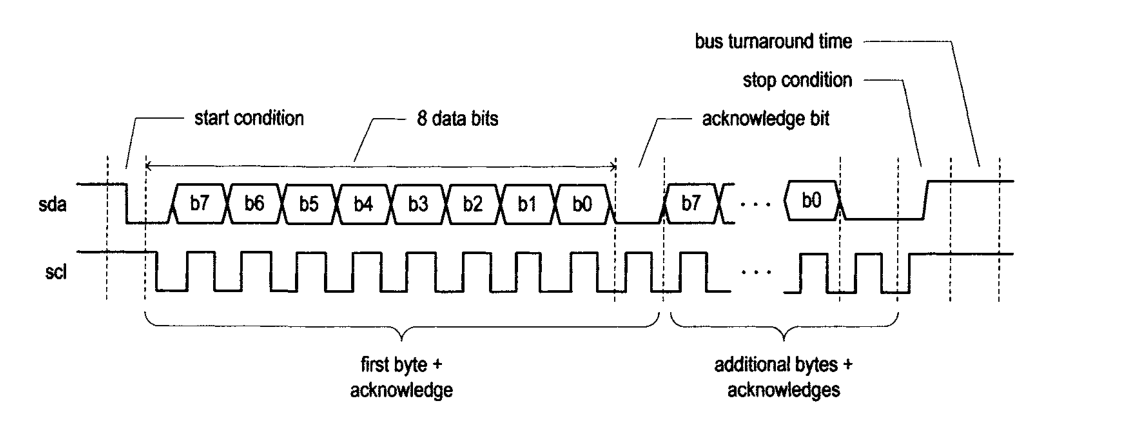
\includegraphics[width=0.8\textwidth]{Imagenes/basic_timing.png}
			\caption{Diagrama de tiempos genérico de una transferencia por $I^{2}C$}
			\label{fig:basic_timing}
		\end{figure} 

			La transferencia esta hecha byte-a-byte con el MSB primero. Cada byte es seguido con un ``acknowledge" bit en el noveno pulso de reloj. El número de bytes en una transferencia no está restringido. Después de terminado, el master finaliza la transferencia creando una condición de parada (P), en la cual SDA cambia de bajo a alto mientras SCL se mantiene en alto. Luego de que la transferencia esta completada el bus debe esperara un pequeño tiempo (turnaround time) antes de inicializar otra transacción.
		
			\paragraph{Características eléctricas.} La conexión del bus $I^{2}C$ se muestra en la figura \textcolor{blue}{\textbf{\ref{fig:electric_char}}}, usa la tecnología ``drenador-abierto", lo que significa que en la etapa de salida de un dispositivo tiene que tener la estructura de drenador-abierto. Tanto la linea \textit{sda} como \textit{scl} están conectadas a $V_{DD}$ a través de las resistencias pull-up las cuales representan un estado en alto cuando el bus esta en alta impedancia. La línea se vuelve en bajo cuando la salida de alguno de los dispositivos se vuelve bajo. Se dice que realiza la función de ``and-cableada".
		\begin{figure}[H]
			\centering
			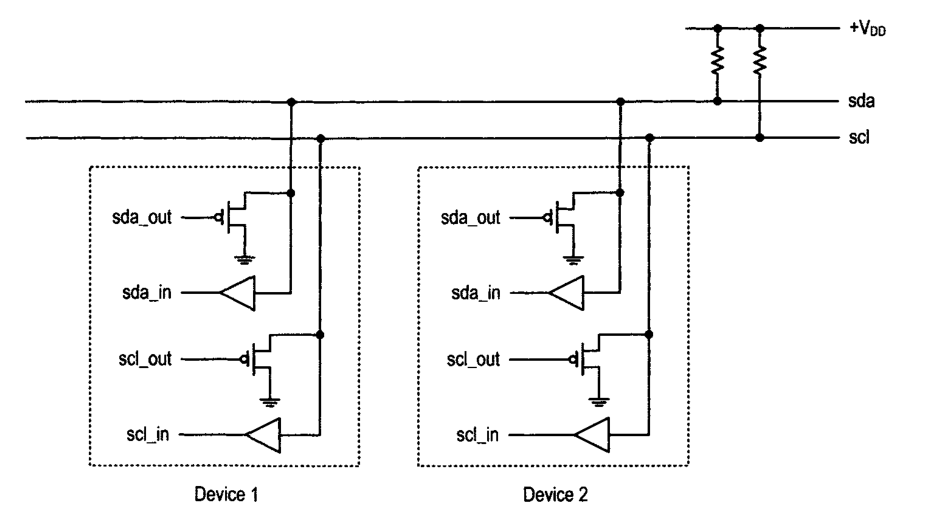
\includegraphics[width=0.6\textwidth]{Imagenes/open-drain.png}
			\caption{Diagrama conceptual de un bus $I^{2}C$.}
			\label{fig:electric_char}
		\end{figure} 
		
		\paragraph{Protocolo de bus.} Cuando el bus esta en \textit{idle}, cualquier dispositivo puede comenzar la transferencia y convertirse en el \textit{master}. Una tipica transferencia de datos esta compuesta de varias partes:
		\begin{itemize}\itemsep 0em
			\item Start.
			\item Dirección del esclavo mas bit de dirección.
			\item Datos.
			\item Stop.
		\end{itemize}
		
		El \textit{master} inicia la condición de \textit{start} y luego envía la dirección de 7-bits del esclavo junto con el bit que indica el sentido del flujo de datos, el cual es un 1 para la operación de lectura (del slave al master) y un 0 para la operación de escritura (del master al slave). El maestro libera la línea de \textit{sda} y el \textit{slave} con la dirección correspondiente debe reconocer tirando a bajo la línea \textit{sda} durante el noveno pulso del reloj. La transferencia de datos puede proceder luego byte-a-byte según lo especificado por el bit de dirección. En la figura \textcolor{blue}{\textbf{\ref{fig:read-write-op}}} se muestran las secuencias completas de escritura y lectura de 2 bytes. Cabe destacar que el master debe generar un bit ``reconocimiento negado" en el noveno ciclo de reloj de la operación de lectura luego de recibir el ultimó byte de datos.

		\begin{figure}[H]
			\centering
			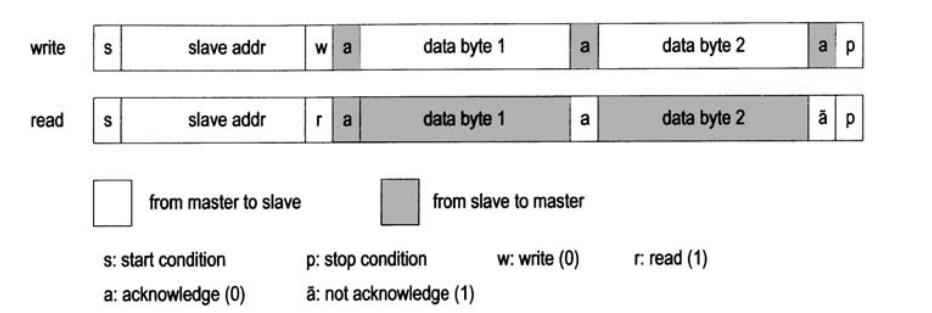
\includegraphics[width=0.8\textwidth]{Imagenes/read-write-op.png}
			\caption{Secuencia completa de escritura y lectura de dos bytes.}
			\label{fig:read-write-op}
		\end{figure} 
	

		\subsubsection{Módulo ds3231.}
			El modulo utilizado es el basado en el integrado RTC ds3231. El ds3231 es un reloj de tiempo real (RTC) extremadamente preciso con un oscilador integrado con compensación de temperatura de cristal (TCXO). El dispositivo incorpora la posibilidad de adicionarle una batería y mantener el cronometraje preciso cunado se interrumpe la alimentación principal del módulo. Ademas incluye una memoria EEPROM AT24C32 de 32Kb y un sensor de temperatura.  

		\begin{figure}[H]
			\centering
			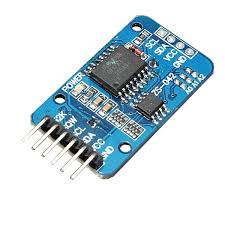
\includegraphics[width=0.2\textwidth]{Imagenes/ds3231.png}
			\caption{Módulo ds3231.}
			\label{fig:basic_timing}
		\end{figure} 

		El módulo tiene la ventaja que ambos dispositivos (memoria y RTC) se comunican a través del protocolo $I^{2}C$, las direcciones de memoria se puede observar en la figura \textcolor{blue}{\textbf{\ref{fig:slave_add}}}, la dirección de memoria es mapeable a dos direcciones posibles debido a una compatibilidad de la susodicha con un modelo anterior de memoria. 

		\begin{figure}[H]
			\centering
			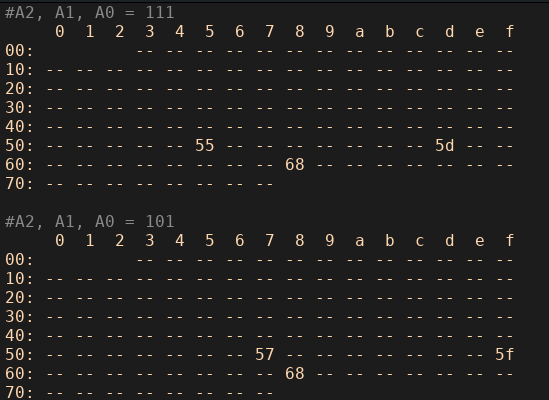
\includegraphics[width=0.4\textwidth]{Imagenes/slave-add.png}
			\caption{Direcciones de memoria en hexadecimal.}
			\label{fig:slave_add}
		\end{figure} 

		La dirección del RTC es 0x68 y la memoria comparte tanto 0x5d como 0x55, esta puede ser modificada cerrando los puentes A0, A1, A2 que se encuentra disponible en el modulo y como se observan en el circuito de la figura \textcolor{blue}{\textbf{\ref{fig:ds3231_sch}}}, de allí que hayan dos tablas de direcciones. 

		\begin{figure}[H]
			\centering
			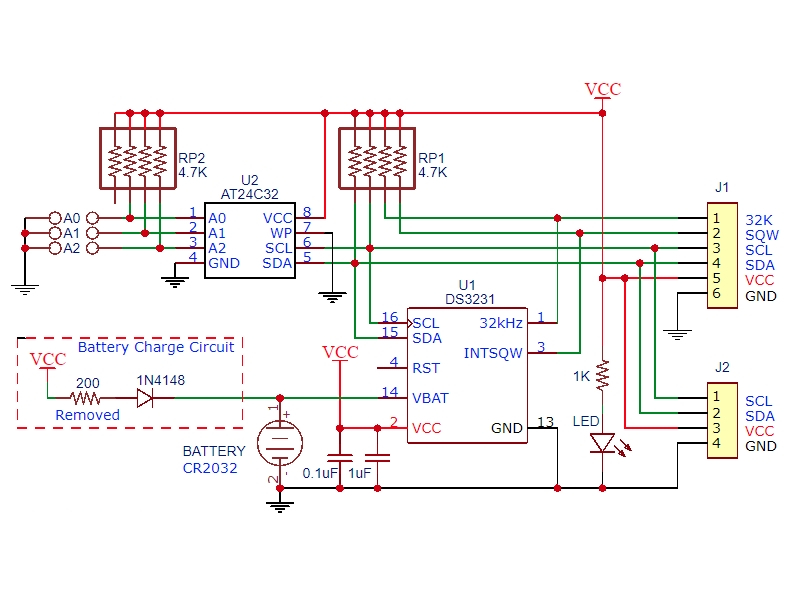
\includegraphics[width=0.6\textwidth]{Imagenes/ds3231-sch.png}
			\caption{Esquemático del módulo.}
			\label{fig:ds3231_sch}
		\end{figure} 

		El PCB está diseñado para que se coloque una pila CR2032 recargable, en caso que se use una que no lo sea es recomendable desoldar o re posicionar el circuito de carga de batería.

	\subsubsection{Estructura del proyecto}
		El proyecto fue desarrollado en el SW Vivado 2019.2.1 ya que se utilizó la plataforma de entrenamiento de Digilent, Basys3.

		\begin{figure}[H]
			\centering
			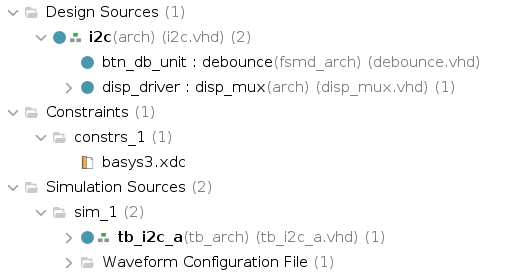
\includegraphics[width=0.6\textwidth]{Imagenes/proy-tree.png}
			\caption{Árbol del proyecto.}
			\label{fig:pry-tree}
		\end{figure} 
	
		\subsection{Protocolo $I^{2}C$}
		Para el desarrollo del protocolo $I^{2}C$ se plantea una maquina de estado que avance deacuerdo a las etapas que indita el datasheet del integrado ds3231 como se ve en la figura \textcolor{blue}{\textbf{\ref{fig:fsm_ds}}}
						
		\begin{figure}[H]
			\centering
			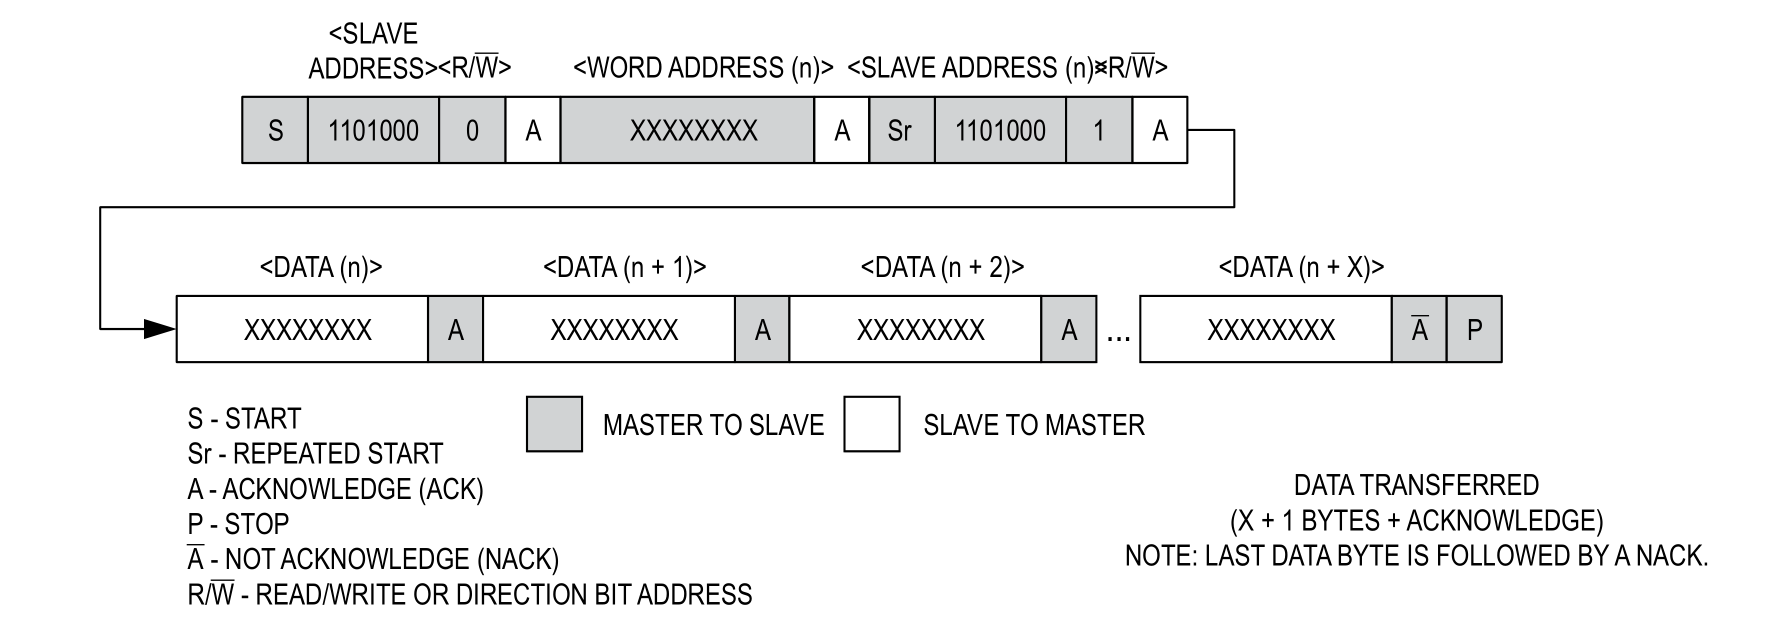
\includegraphics[width=0.8\textwidth]{Imagenes/fsm-ds.png}
			\caption{Secuencia para lectura a partir de un registro del integrado ds3231.}
			\label{fig:fsm_ds}
		\end{figure} 
	
	Las etapas de la máquina de estado planteada es la siguiente:
	\begin{enumerate}\itemsep 0em
		\item La FPGA genera la secuencia de arranque.
		\item Se envía la dirección del slave junto con un 0 para indicar la escritura.
		\item El master espera un ack (0) por parte del slave.
		\item Se envía el registro a escribir.
		\item El master espera un ack (0) por parte del slave.
		\item Sin dejar el bus, se manda una condición de re-start.
		\item Se envía nuevamente la dirección del slave, esta vez junto a un 1 para indicar la operación de lectura.
		\item El master espera un ack (0) por parte del slave.
		\item Se lee un byte transferido por el slave.
		\item El master genera un ack (0).
		\item Los dos anteriores se repite 2 veces mas, salvo que en el último byte el master genera un nack (1).
		\item El master genera la secuencia de stop y libera el bus.
	\end{enumerate}

	Tanto para la generación de datos como de los casos especiales de start, stop la trama se trabaja con un contador, para garantizar el cumplimiento de los tiempos necesarios para la comunicación. En la figura \textcolor{blue}{\textbf{\ref{fig:time_gen}}} se observa como se forman cada una de estas condiciones.


		\begin{figure}[H]
			\centering
			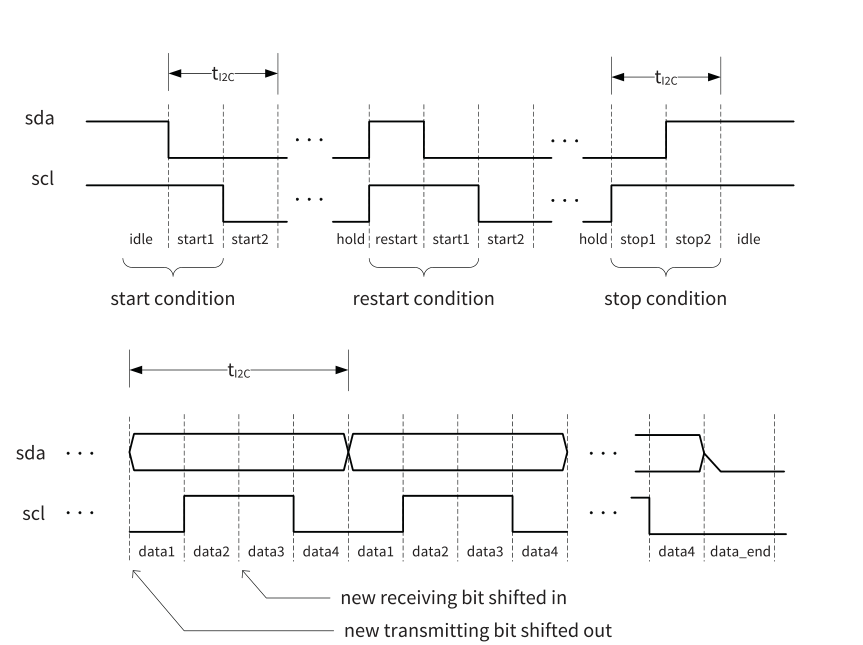
\includegraphics[width=0.6\textwidth]{Imagenes/time-gen.png}
			\caption{Divisiones de los estados del $I^{2}C$}
			\label{fig:time_gen}
		\end{figure} 

		Se trabaja con una velocidad de transmicion de 100 Kb, por este motivo y lo visto previamente se determinan dos constantes \textit{QUTR} y \textit{HALF} que representan respectivamente un cuarto y la mitad de un ciclo de reloj completo.

		\begin{figure}[H]
			\centering
			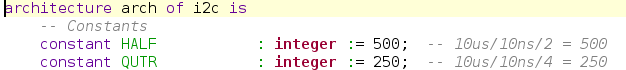
\includegraphics[width=0.6\textwidth]{Imagenes/period.png}
			\caption{Constantes para 100 Kb.}
		\end{figure} 

		Tanto para la escritura como la recepción, los datos se parten en 4 segmentos, como se puede apreciar en la figura \textcolor{blue}{\textbf{\ref{fig:data_proc}}}, esto es para poder construir los flancos ascendentes y descendentes del clock, como así también set capaz de recibir en la mitad del periodo del clock el dato que envíe el slave.

		\begin{figure}[H]
			\centering
			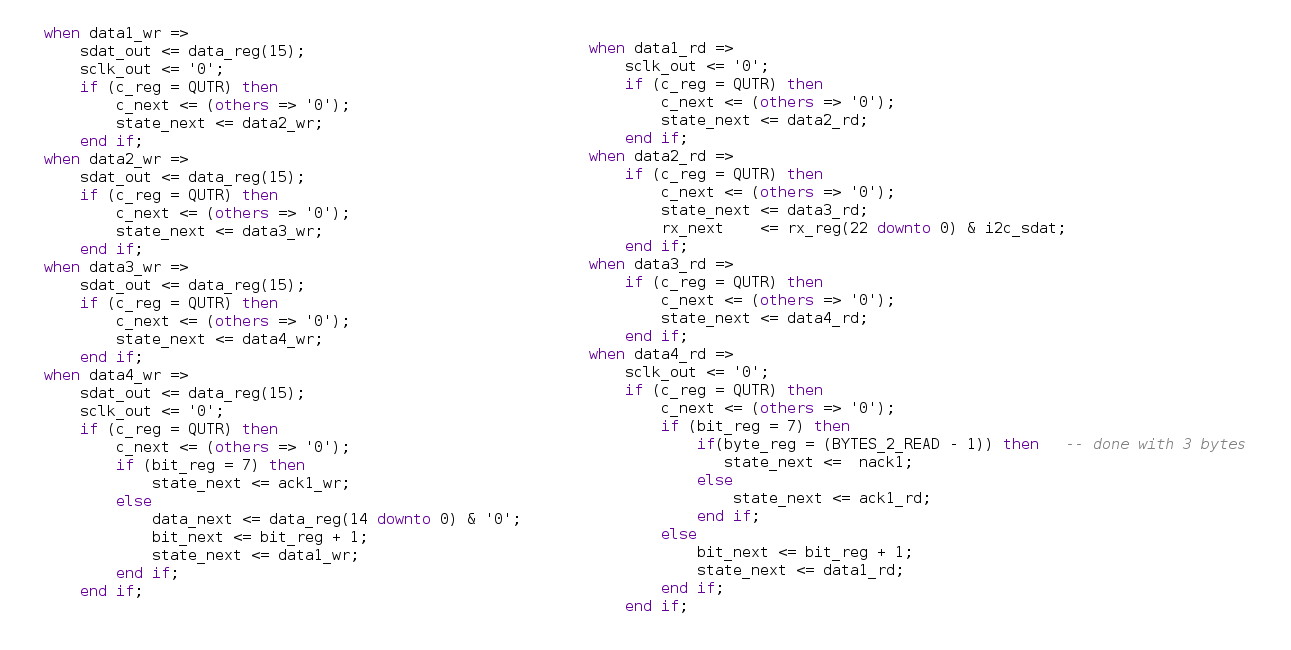
\includegraphics[width=0.8\textwidth]{Imagenes/data_proc.png}
			\caption{Escritura y recepción de datos.}
			\label{fig:data_proc}
		\end{figure} 
		
		\subsubsection{Simulación}
		Para la simulación se simulo la primer trama de envío del address del dispositivo que se va a comportar como slave, para ello se definen como constantes la direccion del address, se utilizan dos registros, uno para escritura y otro para lectura.

		\begin{figure}[H]
			\centering
			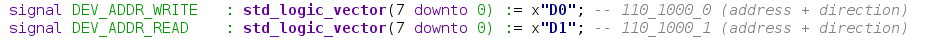
\includegraphics[width=0.8\textwidth]{Imagenes/addr_constant.png}
			\caption{Adress del ds3231 para escritura y lectura.}
		\end{figure} 

		\begin{figure}[H]
			\centering
			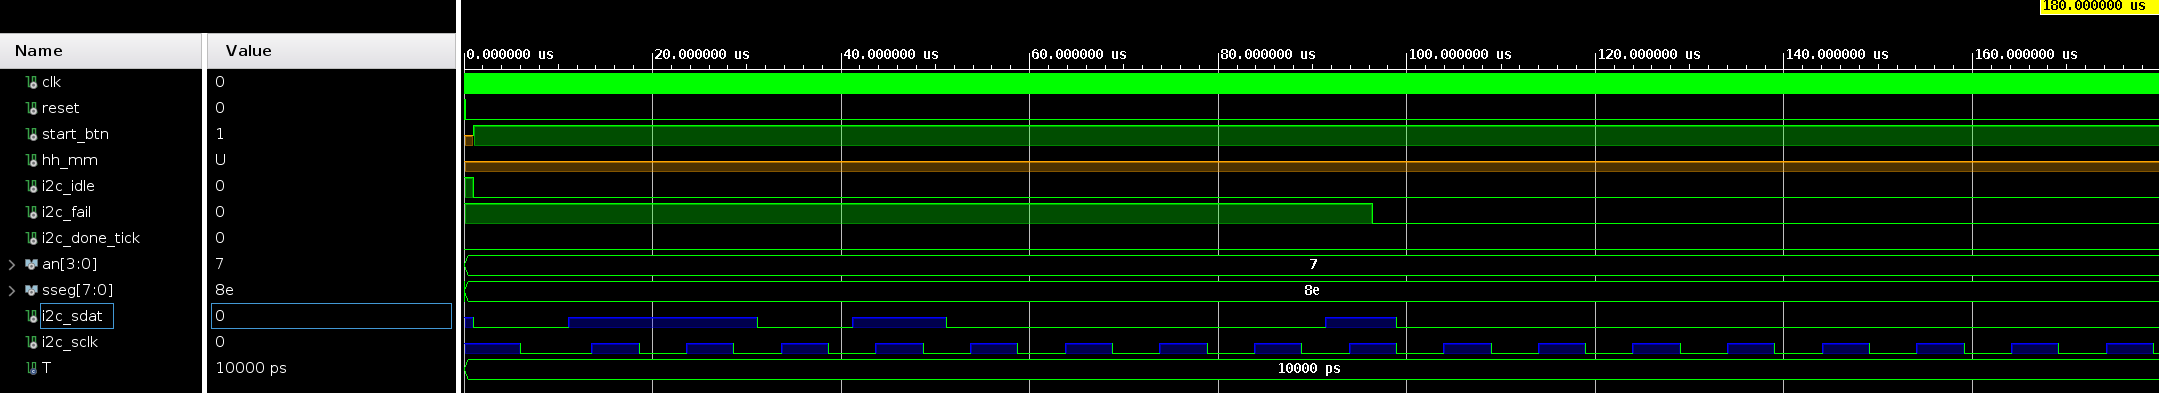
\includegraphics[width=\textwidth]{Imagenes/add_i2c.png}
			\caption{Simulacion del envio del address de escritura.}
		\end{figure} 
\clearpage

		\subsection{Multimedia}
		Se adjunta un dos links de unos vídeos demostrativos: 
		\begin{itemize}
			\item Presentación: \url{https://youtu.be/1az8Dk07Ik4}
			\item Demo: \url{https://youtu.be/NCIMGwVY518}
		\end{itemize}
		
\end{document}
